\begin{frame}{Community Service for free WiFi}
\begin{columns}[c]
    \column{.5\textwidth}
    \begin{itemize}
    \item Purple added a fake clause to its WiFi Terms: \textbf{1,000 hours of community service}.
    \item Tasks included:
    \begin{itemize}
        \item Cleaning toilets at festivals
        \item Hugging stray animals
        \item Scraping gum off streets
    \end{itemize}
    \item Over \textbf{22,000 users accepted}; only \textbf{1 person} noticed.
\end{itemize}

\vspace{0.2cm}
\textit{Goal: Show how blindly users click “I Agree.”} 
    \column{.5\textwidth}
    \centering
    \begin{figure}
        \centering
        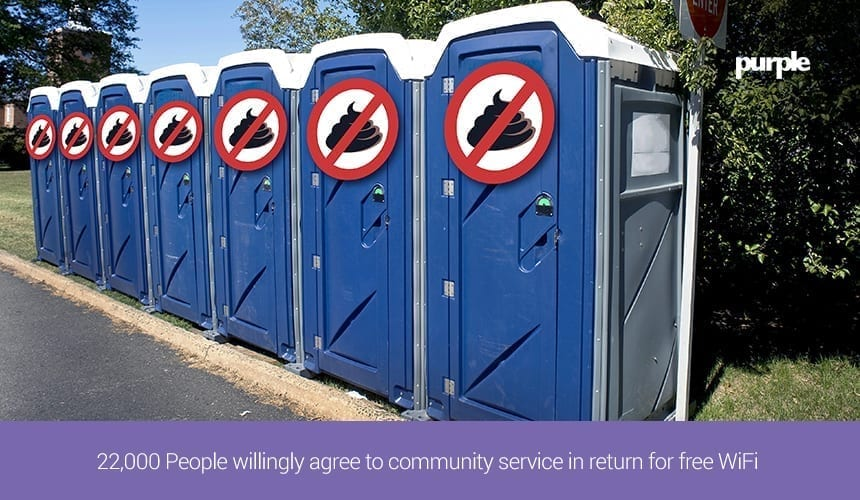
\includegraphics[width=\textwidth]{images/toilet.png}
        \label{fig:toilet}
    \end{figure}    
\end{columns}
\end{frame}

\begin{frame}{Lesson}
\begin{columns}[c]
    \column{.65\textwidth}
    \begin{itemize}
    \item Experiment raised awareness of careless digital consent.
    \item Inspired changes:
    \begin{itemize}
        \item Privacy policy shortened from 1,600 to 260 words.
        \item Clearer data usage explanations.
        \item Launch of a user-controlled Profile Portal \cite{TOILET}.
    \end{itemize}
\end{itemize}
    \column{.35\textwidth}
    \centering
    \begin{figure}
        \centering
        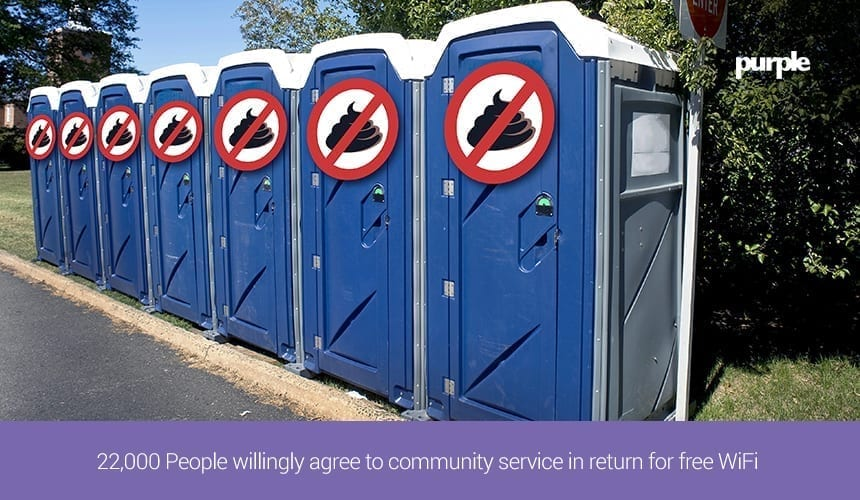
\includegraphics[width=\textwidth]{images/toilet.png}
        \label{fig:toilet}
    \end{figure}    
\end{columns}
\end{frame}

\begin{frame}{The Herod Clause}
\begin{columns}[c]
    \column{.5\textwidth}
  \begin{itemize}
    \item In June 2014, researchers set up public Wi-Fi hotspots in London.
    \item Users had to accept T\&Cs to get access.
    \item One clause (the “Herod Clause”) stated:
    \begin{quote}
        “You agree to assign your first born child to us for the duration of eternity.”
    \end{quote}
    \item \textbf{6 people accepted the terms} without noticing.
    \item Clause was later removed — the children were “returned.”
\end{itemize}

    \column{.5\textwidth}
    \centering
    \begin{figure}
        \centering
        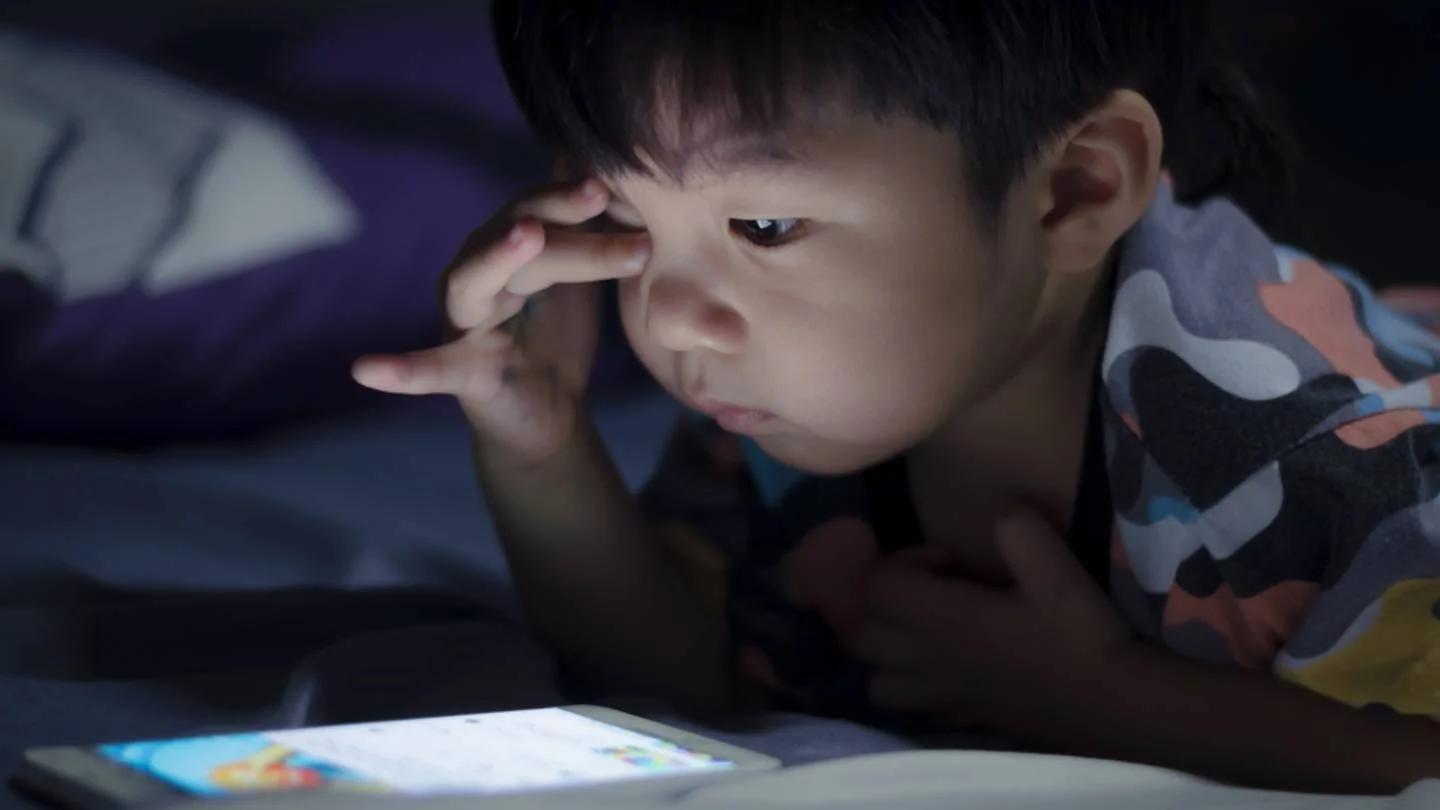
\includegraphics[width=\textwidth]{images/child.png}
        \label{fig:child}
    \end{figure}    
\end{columns}
\end{frame}

\begin{frame}{Why This Matters}
\begin{columns}[c]
    \column{.5\textwidth}
  \begin{itemize}
    \item Experiment run by the Cyber Security Research Institute and F-Secure.
    \item Goal: Raise awareness of careless public Wi-Fi use.
    \item Highlights two key issues:
    \begin{itemize}
        \item \textbf{Blind acceptance} of legal agreements.
        \item \textbf{Lack of awareness} about security risks in public networks\cite{CHILD}.
    \end{itemize}
\end{itemize}

    \column{.5\textwidth}
    \centering
    \begin{figure}
        \centering
        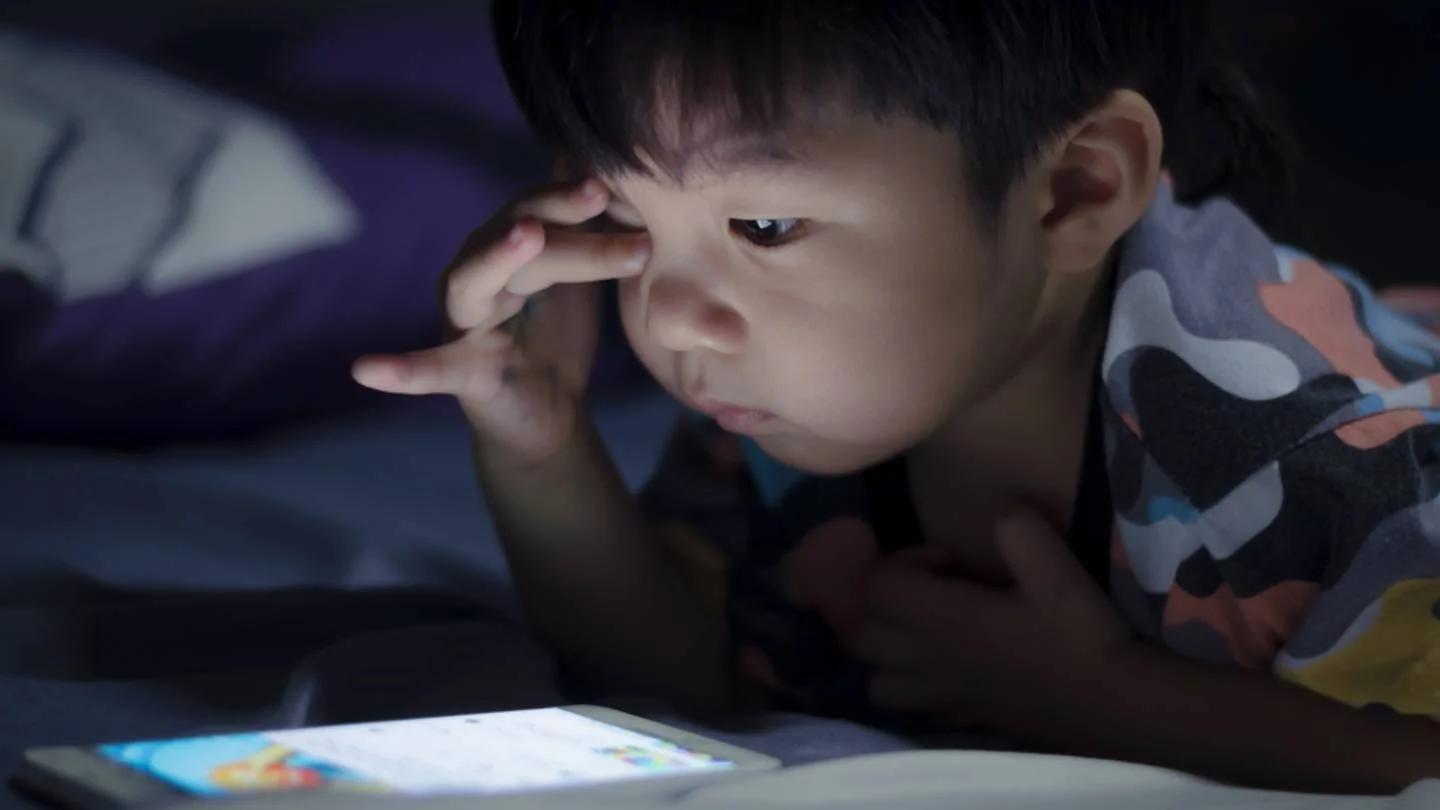
\includegraphics[width=\textwidth]{images/child.png}
        \label{fig:child}
    \end{figure}    
\end{columns}
\end{frame}
